\documentclass[12pt]{article}


\usepackage{Homework}
% \usepackage{minted}

% Creates the header and footer.
\pagestyle{fancy}
\fancyhead[l]{Michael Hoon, $1006617$}
\fancyhead[c]{40.002 Optimisation Problem 1}
\fancyhead[r]{\today}
\fancyfoot[c]{\thepage}
\renewcommand{\headrulewidth}{0.2pt} %Creates a horizontal line underneath the header
\renewcommand{\footrulewidth}{0.2pt}
\setlength{\headheight}{15pt} %Sets enough space for the header
\newcommand{\HRule}[1]{\rule{\linewidth}{#1}}


\begin{document}

% \title{Another fancyhdr demo}
% \author{\texttt{tex.stackexchange} \textit{et al}}
% \maketitle
% \newpage


\title{ \normalsize \textsc{} 
        \\ [2.0cm]
		\HRule{1.5pt} \\
		\LARGE \textbf{\uppercase{40.002 Optimization} 
        \HRule{2.0pt} \\ [0.6cm]
        \LARGE{Problem 1} \vspace*{10\baselineskip}}
		}
\date{\today}
\author{\textbf{Michael Hoon} \\ 1006617}

\maketitle 
\newpage


\section*{Question 1}

a) Let $D$ and $F$ denote Domestic and Foreign stocks (in millions) respectively. We formulate the Linear Program (LP): 

\begin{align*}
    \max_{D, F} \quad & 0.11D + 0.17F \\
    \text{s.t.} \quad & D + F \leq 12 \\ 
    & 0 \leq D \leq 10 \\
    & 0 \leq F \leq 7 \\ 
    & D \geq \frac{1}{2}F \\ 
    & F \geq \frac{1}{2}D 
\end{align*} \\

\noindent b) Graphically, we have Figure \ref{fig:1-feasibleregionlp} with corner points labelled and the feasible region shaded:

\begin{figure}[H]
    \centering
    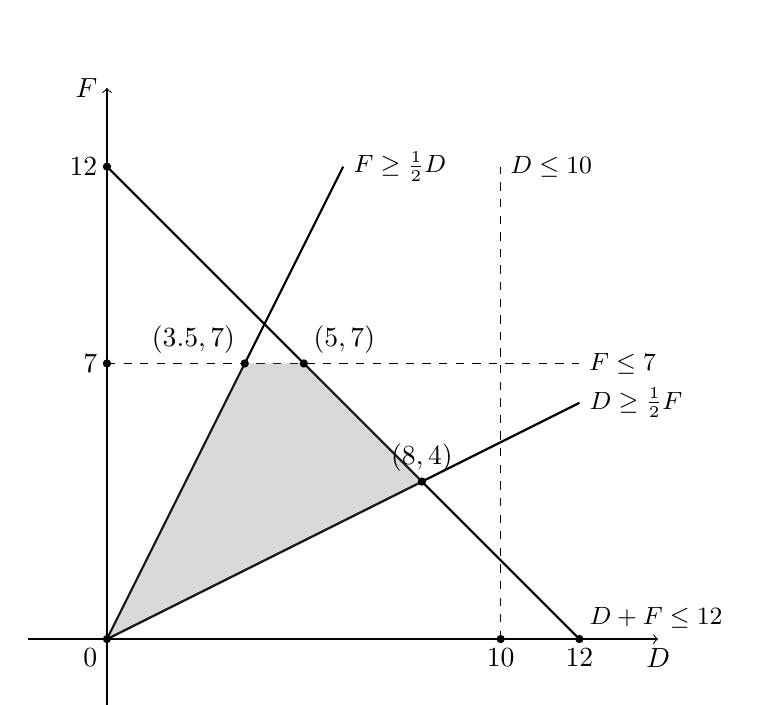
\begin{tikzpicture}[scale=0.5]
        % Draw axes
        \draw[->] (-2,0) -- (14,0) node[below] {$D$};
        \draw[->] (0,-2) -- (0,14) node[left] {$F$};

        % Constraint 1: x + y <= 12
        \draw[thick] (0,12) -- (12,0) node[above right]{\small $D + F \leq 12$};

        % Constraint 2: 0 <= x <= 10
        \draw[dashed] (10,0) -- (10,12) node[right]{\small $D \leq 10$};

        % Constraint 3: 0 <= y <= 7
        \draw[dashed] (0,7) -- (12,7) node[right]{\small $F \leq 7$};

        % Constraint 4: x >= 1/2 y
        \draw[thick] (0,0) -- (12,6) node[right]{\small $D \geq \frac{1}{2}F$};

        % Constraint 5: y >= 1/2 x
        \draw[thick] (0,0) -- (6,12) node[right]{\small $F \geq \frac{1}{2}D$};

        \fill[gray, opacity=0.3] (0,0) -- (3.5,7) -- (5,7) -- (8,4) -- cycle;

        % Corner Points
        \fill (10,0) circle (3pt) node[below] {$10$};
        \fill (8,4) circle (3pt) node[above] {$(8,4)$};
        \fill (5,7) circle (3pt) node[above right] {$(5,7)$};
        \fill (0,7) circle (3pt) node[left] {$7$};
        \fill (0,0) circle (3pt) node[below left] {$0$};
        \fill (0,12) circle (3pt) node[left] {$12$};
        \fill (12,0) circle (3pt) node[below] {$12$};
        \fill (3.5,7) circle (3pt) node[above left] {$(3.5,7)$};
    \end{tikzpicture}
    \caption{Feasible Region of LP}
    \label{fig:1-feasibleregionlp}
\end{figure} 


\noindent c) Solving graphically, the optimal value of $F$ and $D$ that maximises returns are $D = 5$, $F = 7$ from Figure \ref{fig:1-feasibleregionlp}, for a total (maximum) return of:

\begin{equation*}
    \boxed{0.11(5) + 0.17(7) = \$ 1.74 \; \text{million}}
\end{equation*} \\

\noindent To prove that this is the global maximum, we brute-force attempt to find the returns of the other corner points: \\ 

\noindent For $(3.5, 7)$, we have:

\begin{equation*}
    0.11(3.5) + 0.17(7) = \$ 1.575 \; \text{million} < \$ 1.74 \; \text{million}
\end{equation*}

\noindent For $(8, 4)$, we have: 

\begin{equation*}
    0.11(8) + 0.17(4) = \$ 1.56 \; \text{million} < \$ 1.74 \; \text{million}
\end{equation*} \\ 

\noindent And thus $\$ 1.74 \; \text{million}$ is indeed the global maximum return for the fund. 


\newpage 

\section*{Question 2}
a) Given the LP constraints 

\begin{align*}
    -x_{1} + x_{2} & \geq 1 \\ 
    x_{1} & \geq 0
\end{align*}

\noindent We have the feasible region shaded and corner points labelled: 

\begin{figure}[H]
    \centering
    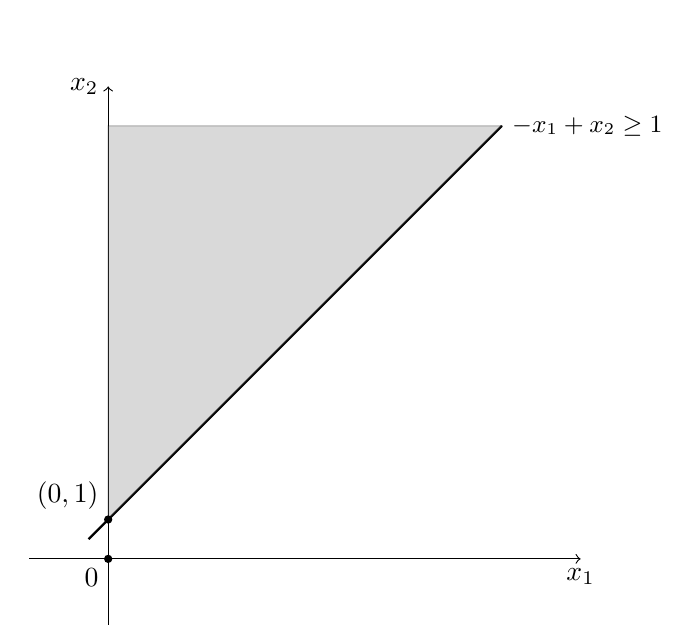
\begin{tikzpicture}[scale=0.5]
        % Axis
        \draw[->] (-2,0) -- (12,0) node[below]{$x_1$};
        \draw[->] (0,-2) -- (0,12) node[left]{$x_2$};

        % Constraint 1
        \draw[thick] (-0.5,0.5) -- (10,11) node[right]{\small $-x_1 + x_2 \geq 1$};

        % Feasible Region
        \filldraw[fill=gray, opacity=0.3] (0,1) -- (0,11) -- (10,11) -- cycle;

        % Corner Points
        \fill (0,1) circle (3pt) node[above left] {$(0,1)$};
        \fill (0,0) circle (3pt) node[below left] {$0$};
    \end{tikzpicture}
    \caption{Feasible Region of LP}
    \label{fig:2-feasiblelp2}
\end{figure} 

\noindent b) For a minimisation problem, we have the complete LP: 

\begin{align*}
    \min_{x_{1}, x_{2}} \quad & \alpha x_{1} + x_{2} \\ 
    \text{s.t.} \quad &-x_{1}+x_{2} \geq 1 \\
    & x_{1} \geq 0
\end{align*}

\noindent i) For the optimal solution to be unique, we need $\alpha = 0$ for a minimum at $x_{2} = 1$. \\ 

\noindent ii) For there to be multiple optimal solutions with infinite optimal objective values, we need $\alpha \in \mathbb{R} \backslash \{-1,0\}$. \\ 

\noindent iii) For there to be an unbounded optimal objective value, we need $\alpha = -1$. 

\newpage 

\section*{Question 3}
a) Since $Z$ is a discrete random variable that takes values in the set $\{1, 2, \dots, 10\}$, and $p_i = \text{Prob}(Z = i) \; \forall i \in \{1, 2, \dots , 10\}$, with sum and non-negative constraints, we can formulate the LP: 

\begin{align*}
    \max_{p_i} \quad & \sum_{i=5}^{10} p_i \\ 
    \text{s.t.} \quad & \sum_{i=1}^{10} p_i = 1 \\ 
    & \sum_{i=1}^{10} i \cdot p_i = 4 \\ 
    & p_i \geq 0
\end{align*}

\noindent We want to optimise the probability distribution of $Z$ such that the likelihood of $Z$ being 5, 6, 7, 8, 9, or 10 is maximised. \\ 

\noindent Using the following \textit{JuMP} code, we have the final probability distribution of $Z$ being: 

\begin{equation*}
    \boxed{p = \{0.25, 0, 0, 0, 0.75, 0, 0, 0, 0, 0\}}
\end{equation*}

% \begin{minted}{Julia}
%     using JuMP
%     using GLPK
    
%     model = Model(GLPK.Optimizer)
    
%     # Decision variables
%     @variable(model, p[1:10] >= 0)
    
%     # Objective function
%     @objective(model, Max, sum(p[5:10]))
    
%     # Normalization constraint
%     @constraint(model, sum(p) == 1)  
%     # Average value constraint
%     @constraint(model, sum(i * p[i] for i in 1:10) == 4)  
    
%     # Solving LP
%     optimize!(model)

%     optimal_probabilities = value.(p)
%     println("Optimal Probability Distribution: ", optimal_probabilities)
% \end{minted}

\newpage

\newpage

\section*{Question 4}
For the minimisation problem: 

\begin{align*}
    \min \quad & x_{1}-x_{2} \\ 
    \text{s.t.} \quad & 2 x_{1} + 3 x_{2} - x_{3} + x_{4} \leq 0 \\ 
    & 3 x_{1} + x_{2} + 4 x_{3} - 2 x_{4} \geq 3 \\ 
    & - x_{1} - x_{2} + 2 x_{3} + x_{4} = 6 \\ 
    & x_{1} \leq 0 \\ 
    & x_{2},\; x_{3} \geq 0 
\end{align*}

\noindent We can rearrange the LP into the form: 

\begin{align*}
    \max \quad & \mathbf{c}^{\top} \mathbf{x} \\ 
    \text{s.t.} \quad & \mathbf{A} \mathbf{x} \leq \mathbf{b}
\end{align*}

\noindent For the $3^{\text{rd}}$ constraint, we separate into two cases: 

\begin{align*}
    - x_{1} - x_{2} + 2 x_{3} + x_{4} & \geq 6 \\
    x_{1} + x_{2} -2 x_{3} -x_{4} & \leq -6
\end{align*}

\noindent where:

\begin{equation*}
    \mathbf{x} = \begin{bmatrix}
        x_{1} \\ x_{2} \\ x_{3} \\ x_{4} 
    \end{bmatrix},
    \quad 
    \mathbf{c} = \begin{bmatrix}
        1 \\ -1 \\ 0 \\ 0
    \end{bmatrix},
    \quad 
    \mathbf{A} = \begin{bmatrix}
        2 & 3 & -1 & 4 \\ 
        -3 & -1 & -4 & 2 \\ 
        -1 & -1 & 2 & 1 \\ 
        1 & 1 & -2 & -1 \\ 
        1 & 0 & 0 & 0 \\ 
        0 & -1 & 0 & 0 \\ 
        0 & 0 & -1 & 0 
    \end{bmatrix},
    \quad 
    \mathbf{b} = \begin{bmatrix}
        0 \\ -3 \\ 6 \\ -6 \\ 0 \\ 0 \\ 0
    \end{bmatrix}
\end{equation*}

\newpage 
\section*{Question 5}
The given optimisation problem is non-linear in nature, due to the piecewise absolute value function $f(z)$ in the objective function. We linearise the problem by introducing additional constraints and auxiliary variables. Let $y_i$ be auxiliary variables for each $i$, and $z_i$ be the absolute value of $\mathbf{a}^{\top}_i \mathbf{x}- b_i$. \\

\noindent Enforcing additional constraints to the problem in place of the piecewise nonlinear $f(x)$ in the objective function, we now formulate an appropriate LP:

\begin{align}
    \nonumber \min \quad & \sum_{i=1}^{m} y_i \\ 
    \text{s.t.} \quad & z_i = \mathbf{a}^{\top}_i \mathbf{x} - b_i, \quad i = 1, \dots , m \\ 
    & y_i \geq z_i - 5,  \quad i = 1, \dots , m \\ 
    & y_i \geq -(z_i - 5), \quad i = 1, \dots , m \\ 
    & y_i \geq 0, \quad i = 1, \dots , m  \\
    & \mathbf{x} \in \mathbb{R}^{n} 
\end{align}

\noindent Constraint (2) enforces a lower bound on the LP, in view of the first piece of $f(z)$ where it is $0$ when $|z| < 5$. Constraint (3) enforces an upper bound, in view of the second piece of $f(z)$ for $|z| \geq 5$. Lastly, the non-negativity constraint (4) is imposed to ensure the absolute value of $z_i$.  

\section*{Question 6}
We are given that $f(\mathbf{x})$ is convex, and we need to show that $\forall t \in \mathbb{R}$, the set of $\mathbf{x}$ (denoted by $\chi_t$) that satisfies $f(\mathbf{x}) \leq t$ is a convex set. Geometrically, for any 2 points $\mathbf{x}_1$ and $\mathbf{x}_2$ in $\chi_t$, the line segment containing them must also be in $\chi_t$. i.e., if $\mathbf{x}_1, \mathbf{x}_2 \in \chi_t$, then $\lambda \mathbf{x}_1 + (1-\lambda)\mathbf{x}_2 \in \chi_t, \; \forall \lambda \in [0,1]$. \\ 

\begin{proof}
    $ $ \newline $\because \mathbf{x}_1, \mathbf{x}_2 \in \chi_t$, then $f(\mathbf{x}_1) \leq t$ and $f(\mathbf{x}_2) \leq t$. Since $f(\mathbf{x})$ is convex, we use the property: \\ 
    \begin{align*}
        f(\lambda \mathbf{x}_1 + (1-\lambda) \mathbf{x}_2) & \leq \lambda f(\mathbf{x}_1) + (1-\lambda) f(\mathbf{x}_2) \\ 
        & \leq \lambda t + (1- \lambda) t \\ 
        &= \lambda t + t - \lambda t \\ 
        &= t
    \end{align*}

    \noindent $\therefore \; \forall \lambda \in [0,1], \; f(\lambda \mathbf{x}_1 + (1-\lambda) \mathbf{x}_2) \leq t$, and thus $\lambda \mathbf{x}_1 + (1-\lambda) \mathbf{x}_2 \in \chi_t$, which is convex.  
\end{proof}


\noindent An appropriate illustration of this is Figure \ref{fig:6-convexfns} below. 

\begin{figure}[H]
    \centering
    \includegraphics[width=0.7\textwidth]{Images/convexityfn.png}
    \caption{Illustration of Convexity}
    \label{fig:6-convexfns}
\end{figure} 

\section*{Question 7}

\subsection*{(1)}
\begin{align*}
    \max \quad & 5x_{1} x_{2} + 12 x_{3} \\ 
    \text{s.t.} \quad & x_{3} \leq 2 \\ 
    & x_{2} \leq 5 \\ 
    & 3.2 x_{2} + 5.1 x_{1} = 5.1 \\ 
    & x_{1} + \log x_{2} - x_{3} = 0 \\ 
    & x_{1}, x_{2}, x_{3} \in \{0,1\}
\end{align*}

\noindent For this LP, Proportionality, Additivity, and Certainty assumptions hold, while Divisibility does not. The final constraint suggests that $x_{1}, x_{2}, x_{3}$ are constrained to values either 0 or 1 in the set, which are only binary whole numbers, and not fractional values. 

\subsection*{(2)}

\begin{align*}
    \max \quad & 5x_{1} - x_{2} - 2 x_{3} \\ 
    \text{s.t.} \quad & x_{3} \leq 2.9 \\ 
    & x_{2} \geq \theta \\ 
    & x_{3} + x_{2} - x_{1}^{2} = 0 \\ 
    & 0.4 \frac{x_{1}}{x_{2}} + x_{3} \leq  0 \\ 
    & x_{1}, x_{2}, x_{3} \geq 0 \\ 
    & \theta \in U(0,1)
\end{align*}

\noindent For this LP, Proportionality, Additivity, hold, while Divisibility and Certainty do not. For Divisibility, the constraint involving the random variable $\theta \in U(0,1)$ does not explicitly imply that the decision variable $x_2$ can be assigned to fractional values. For Certainty, since random variables are stochastic in nature, there is no way to know for sure the value of $x_2$. 

\subsection*{(3)}


\begin{align*}
    \max \quad & x_{1} - 15x_{2} - 10 x_{3} \\ 
    \text{s.t.} \quad & \frac{x_{3}}{x_{2}} \leq 20 \\ 
    & x_{2} - 4 x_{1} \leq 0 \\ 
    & x_{3} + x_{2} - x_{1} = 0 \\ 
    & x_{1}, x_{2}, x_{3} \geq 0 \\ 
\end{align*}

\noindent For this LP, all 4 assumptions of Proportionality, Additivity, Divisibility, and Certainty hold. 


\end{document}
